\documentclass[a4paper,11pt]{article}

\usepackage[french]{babel}
\usepackage[T1]{fontenc}
\usepackage[utf8]{inputenc}
\usepackage{changepage}
\usepackage{graphicx}
%\usepackage{fullpage}

\begin{document}

\title{\textbf{Compte-rendu de travaux pratiques}\\Traitement du signal}
\author{Thibaut Castanié\\\textit{Master IMAGINA}}
\date{Décembre 2014}

\maketitle

\thispagestyle{empty}

\newpage 
\section*{Introduction}
Ces travaux pratiques ont pour but de manipuler des signaux audio sur le plan fréquentiel et temporel. Pour mener à bien ces projets, deux fichiers Wave.cpp et Wave.hpp sont à disposition pour lire et créer des fichiers audio au format \texttt{.wav}. Des fichiers son, enregistrés en mono-voie, sont aussi à disposition afin d'effectuer des tests durant le différentes phases des travaux pratiques.\\
Le but de ces petits projets étant de comprendre le fonctionnement d'un signal audio et les opérations réalisables dessus afin d'en faciliter sa transmission.
\newpage 
\section{Prise en main des signaux}
Dans un premier temps, il est nécessaire de bien comprendre le fonctionnement du fichier Wave.cpp permettant de manipuler les fichier audio de type WAV. En ouvrant un fichier audio sous le logiciel Audacity, on visualise facilement de quoi est vraiment composé le signal. En agrandissant le signal, on constate que ce dernier est composé d'une multitudes de points placés à une certaine hauteur sur la piste.

\begin{center}
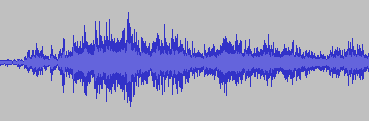
\includegraphics[scale=1]{zoom1.png}\\
\textit{Fichier audio sous Audacity}
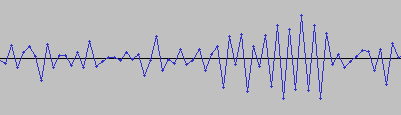
\includegraphics[scale=1]{zoom2.png}\\
\textit{Zoom sur une partie du signal, sous Audacity}
\end{center}

\paragraph{} La représentation simple d'Audacity permet de comprendre plus facilement la structure et le fonctionnement du fichier Wave.cpp qui manipule des fichier du même type. Il contient donc des informations telles que la taille du chier, son codage en bits, son échantillonnage, ainsi que le tableau contenant les informations sur le signal sonore en question.

\paragraph{} Une fois la compréhension faite, il faut passer à la manipulation. Pour cela, l'exercice le plus simple est de créer une copie d'un fichier \texttt{.wav} existant. On récupère les informations contenues dans le fichier qu'on stocke dans des variables locales, puis on les réécris à l'identique dans un nouveau fichier. Ensuite, on s'amuse à effectuer des modifications sur les données (la fréquence par exemple), afin de se familiariser avec l'utilisation des fichiers. Cet exercice permet de réaliser les premières manipulations sur les fichiers audio et d'assurer un fonctionnement du code sans erreurs pour la suite des prochains travaux à réaliser.

\section{Création de La.wav}
L'objectif suivant est de créer un fichier audio. Pour cela, la sonorité "La" semble approprié au vu de sa popularité dans nos diapasons et systèmes téléphoniques. Le "La" possède une fréquence de 440Hz. Pour la créer, il faut utiliser la fonction sinus sur un nombre de cycles défini.

\paragraph{} Ainsi, dans une boucle allant de 0 jusqu'au nombre de bits voulu dans le fichiers, on calcule chaque point à l'aide de la fonction \texttt{sin}. La taille du fichier augmente de 1 bit à chaque passage dans la boucle.

\begin{center}
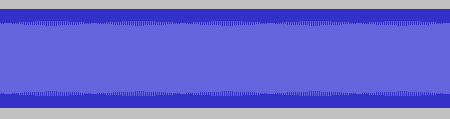
\includegraphics[scale=1]{zoom3.png}\\
\textit{Aperçu du La.wav sous Audacity}
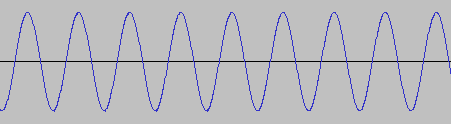
\includegraphics[scale=1]{zoom4.png}\\
\textit{Zoom sur le La.wav, sous Audacity}
\end{center}
\newpage 
\section*{Conclusion}
Ces différents travaux ont permis de manipuler et créer de signaux sonores. Ils permettent aussi de comprendre la dimension mathématique présente dans ceux-ci. L'utilisation de fonctions mathématiques permet de modifier le signal afin de faciliter sa transmission
\bigskip
\bigskip
\bigskip
\bigskip
\bigskip
\bigskip
\subsection*{Note}
N'ayant pas réussi à obtenir un résultat satisfaisant sur le travail effectué sur la transformée de Fourier ainsi que le filtre convolutif causal, j'ai pris la décision de ne pas en parler dans ce compte-rendu.



\end{document}